% vim: set textwidth=78 autoindent:

\section{Plugins di QGIS}\label{sec:plugins}\index{plugins}

% when the revision of a section has been finalized, 
% comment out the following line:
%\updatedisclaimer

Quantum GIS è stato progettato con un'architettura a plugins. Ciò permette di aggiungere nuove caratteristiche e funzioni all'applicazione. Molte delle caratteristiche in QGIS sono in effetti implementate come plugins di base \textbf{Core} o contribuiti dagli utenti \textbf{Esterni}.\index{plugins!types} 

\begin{itemize}
\item \textbf{Plugins Core} sono mantenuti dal team di sviluppo di QGIS e fanno parte automaticamente di ogni distribuzione di QGIS.
Sono scritti in uno dei due linguaggi: C++ or Python.
Ulteriori informazioni riguardanti i plugins core sono disponibili nella sezione  \ref{sec:core_plugins}.
\item \textbf{Plugins esterni} sono attualmente tutti scritti in Python.
Sono immagazzinati in archivi dei pacchetti esterni e mantenuti dai singoli autori.
Possono essere aggiunti a QGIS usando il plugin core chiamato \filename{Plugin Installer}.
Ulteriori informazioni riguardanti i plugins esterni sono disponibili nella sezione \ref{sec:external_plugins}.
\end{itemize}

\subsection{Gestire i Plugins}\label{sec:managing_plugins}
\index{plugins!managing} 

La gestione dei plugins consiste nella loro abilitazione o disabilitazione usando il plugin \filename{Plugin Manager}.
I plugin esterni devono prima essere istallati usando  il plugin \filename{Plugin Installer}.

\subsubsection{Abilitare un Plugin Core}\label{sec:load_core_plugin} 

L'abilitazione di un Plugin Core si ottiene dal menù principale \mainmenuopt{Plugins} > \dropmenuopttwo{mActionShowPluginManager}{Manage Plugins...}.\index{plugins!manager}

\begin{figure}[ht]
   \begin{center}
   \caption{Plugin Manager \nixcaption}\label{fig:pluginmanager}\smallskip
   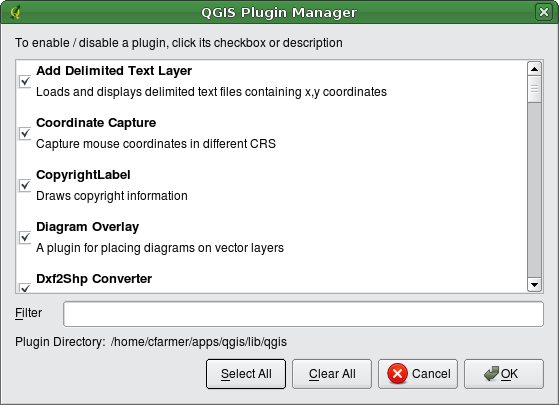
\includegraphics[clip=true, width=14cm]{pluginmanager}
\end{center}
\end{figure}

Il Gestore dei Plugins (Plugin Manager) elenca tutti i plugins disponibili e il loro stato (abilitato o disabilitato).
Tutti i plugins disponibili comprende sia tutti i Core sia tutti gli Esterni che sono stati aggiunti usando il plugin \filename{Plugin Installer} (vedere la sezione \ref{sec:external_plugins}).
la figura \ref{fig:pluginmanager} mostra la finestra di dialogo del Gestore dei Plugin.
I plugin abilitati vengono "ricordati" quando si esce dall'applicazione e riabilitati la prossima volta che QGIS viene lanciato.

\begin{Tip}\caption{\textsc{Il Crash dei Plugins}}\index{crashes}
\qgistip{Se vi accorgete che QGIS va in crash all'avvio, la colpa potrebbe essere di un plugin.
Potete bloccare il caricamento di tutti i plugins attraverso l’editing del suo file di settaggio (vedere \ref{subsec:gui_options} per il settaggio).
Individuate il settaggio dei plugins e cambiate i valori di tutti i plugins su 'false' in modo da impedire il loro caricamento.
\nix {Per esempio, per prevenire il caricamento del plugin \usertext{Delimited text}, la modifica da effettuare sul file  \$HOME/.config/QuantumGIS/qgis.conf di Linux dovrebbe apparire così:\usertext{Add Delimited Text Layer=false}.}
\normalfont 
Farlo per ogni plugin nella sezione Plugins. Quindi avviare QGIS ed aggiungere i plugins
uno alla volta dal Plugin Manager per determinare quale sta causando il problema.
}
\end{Tip} 

\subsubsection{Caricamento di un plugin esterno di QGIS}\label{sec:load_external_plugin} 

Per integrare i Plugins Esterni in QGIS si deve prima caricare il plugin \filename{Plugin Installer} come descritto nella sezione \ref{sec:load_core_plugin}.
Successivamente si possono caricare i Plugins Esterni Python in due passi: 

\begin{enumerate}
\item Scaricare il Plugin Esterno dall'archivio dei pacchetti usando  \filename{Plugin Installer} (Sezione \ref{sec:python_plugin_installer}).
Il nuovo Plugin Esterno verrà aggiunto all alista dei Plugins disponibili nel \filename{Plugin Manager}.
\item Caricare il Plugin usando il \filename{Plugin Manager}.
\end{enumerate}

\subsubsection{Uso dell'Istallatore di Plugins Python }\index{plugins!installing}\label{sec:python_plugin_installer}
\index{plugins!Python Plugin Installer}\index{plugins!upgrading}

\begin{figure}[ht]
   \begin{center}
   \caption{Istallazione di Plugin Esterni Python \nixcaption}
\label{fig:plugininstaller}\smallskip
   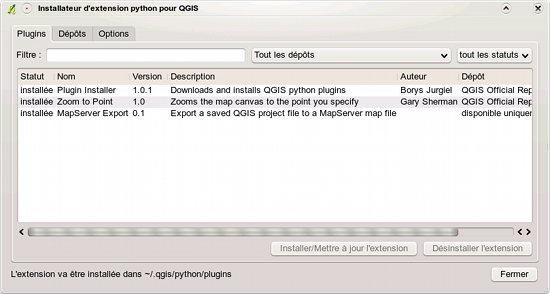
\includegraphics[clip=true, width=14cm]{plugininstaller}
\end{center}
\end{figure}

Per scaricare e istallare un Plugin Python Esterno, selezionare il menuù \mainmenuopt{Plugins} > \dropmenuopttwo{plugin_installer}{Fetch Python Plugins...}.
Apparirà la finestra \filename{Plugin Installer}  (figure \ref{fig:plugininstaller}) con il tab \tab{Plugins}, contenente la lista sia di tutti i Plugins Python disponibili negli archivi remoti sia di quelli istallati. Ogni plugin può essere:
\begin{itemize}
\item \textbf{not installed} - significa che il plugin è disponibile nell'archivio remoto, ma non ancora istallato. Per istallarlo, selezionarlo dalla lista e premere il pulsante  \button{Install plugin}.
\item \textbf{new} - idem come sopra, ma il plugin è visto per la prima volta.
\item \textbf{installed} - il plugin è istallato. Se è anche disponibile in qualsiasi archivio remoto il pulsante \button{Reinstall plugin} è abilitato. Ma la versione disponibile in remoto è più vecchia di quella istallata, appare invece il pulsante \button{Downgrade plugin}.
\item \textbf{upgradeable} - il plugin è istallato, ma è disponibile una versione più recente. Il pulsante \button{Upgrade plugin} è abilitato.
\item \textbf{invalid} - il plugin è istallato, ma è inutilizzabile. La ragione è spiegata nella descrizione del plugin.
\end{itemize}

\minisec{Plugins tab}

Per istallare un plugin, selezionarlo dalla lista e premere il pulsante  \button{Install plugin}. Il plugin è istallato nella sua propria directory, per esempio per \nix sotto \filename{\$HOME/.qgis/python/plugins} ed è visibile solo per l'utente che lo ha istallato. Vedere una lista di altre subdirectories usate per i plugins specifiche per ogni sistema operativo nella Sezione~\ref{subsec:pyfoursteps}. Se l'istallazione va a buon fine, compare un messaggio di conferma. A questo punto andare su \mainmenuopt{Plugins} > \dropmenuopttwo{mActionShowPluginManager}{Manage Plugins...} e caricare il plugin istallato.

Se l'istallazione fallisce, ne viene indicata la ragione. I problemi più frequenti sono correlati a errori di connessione e moduli Python mancanti. Nel primo caso bisognerà attendere alcuni minuti o anche ore, nel secondo è necessario istallare ne sistema operativo i moduli mancanti  prima di usare il plugin. \nix{In Linux, i moduli più richiesti dovrebbero essere disponibili nel gestore dei pacchetti}. \win{Per istruzioni sull'istallazione in Windows, visitare la homepage del modulo}. Se si usa un proxy, può essere necessario configurarlo nel menuù \mainmenuopt{Settings} > \dropmenuopttwo{mActionOptions}{Options} nella tab \tab{Proxy}.

Il pulsante \button{Uninstall plugin} è abilitato solo se il plugin selezionato e istallato e non è un plugin Core. Da notare che se si è istallato un aggiornamento (update) di un Core plugin, si può sempre disistallare tale aggiornamento con il pulsante \button{Uninstall plugin} e ritornare alla versione contenuta nel pacchetto di istallazione di Quantum GIS. Questa non può essere disistallata.

\minisec{Repositories tab}

Il secondo tab \tab{Repositories} contiene una lista di archivi di plugins disponibili per il Plugin Installer. Per impostazioni di default, viene usato solamente l'archivio ufficiale di QGIS (QGIS Official Repository). Si possono aggiungere archivi contribuiti dagli utenti, incluso l'archivio centrale 'QGIS Contributed Repository' ed alcuni altri archivi usando il pulsante \button{Add 3rd party repositories} . Questi archivi contengono un gran numero di più o meno utili plugins ma bisogna tener presente che non sono mantenuti dal Team di Sviluppo di QGIS, che quindi non se ne assume la responsabilità.
Si può anche gestire la lista dei plugins manualmente, cioè aggiungere, rimuovere o editare le singole voci. E' possibile disabilitare temporaneamente un particolare archivio usando il pulsante \button{Edit...}.

La casella di scelta \checkbox{Check for updates on startup} fa sì che QGIS cerchi gli aggiornamenti e le news dei plugins. Se la funzione è selezionata tutti gli archivi elencati e abilitati nella tab \tab{Repositories} sono verificati ogni volta che il programma viene aperto. Se è disponibile un nuovo plugin o l'aggiornamento di uno di quelli già istallati, compare una messaggio di notifica selezionabile nella Barra di Stato. Se la casella di scelta non è selezionata, la ricerca di nuovi plugins e di aggiornamenti viene effettuata solamente quando si lancia il Plugin Installer dal menuù.

Nel caso di problemi con la connessione internet, può esser visibile durante l'intera sessione di QGIS un indicatore  \textit{Looking for new plugins...} nella Barra di Stato e può causare il crash del programma alla chiusura. In questo caso deselezionare la casella di scelta.

\subsection{Data Providers}\index{data providers}

I Data Providers sono plugins speciali che danno accesso ad un archivio di dati. Per default, QGIS supporta i livelli (layers) PostGIS e gli archivi di dati su disco supportati dalla libreria  GDAL/OGR (Appendice \ref{appdx_ogr}).
Un plugin Data Provider estende l'abilità di QGIS di utilizzare altre sorgenti di dati.

I plugins Data Provider sono registrati automaticamente all'avvio di QGIS. Essi non sono gestiti dal Plugin Manager, ma usati dietro le quinte quando un tipo di dati viene aggiunto come livelli in QGIS.
